\section{Computation Review}
\begin{frame}{Computation Review}
\begin{itemize}
\item use factorisation theorem: $s\to \xi S_h$ + PDF
\item $\Pg(k_1) + \Pggx(q) \to \PaQ(p_2) + \PQ(p_1)$
\item three massive particles: $2\cdot m^2>0,q^2=-Q^2<0$
\item compute 2-to-3-phase space: e.g. $dPS_3 \sim dt_1ds_4d\Omega_n$
\item compute diagrams: \includegraphics[width=.2\textwidth]{pyfeyn2/nlo-q-4} + \includegraphics[width=.2\textwidth]{pyfeyn2/nlo-q-3}
\item $\Rightarrow 2xg_1(x) \sim e_u^2\cdot \xi\Delta u(\xi) \otimes d_{P,q}^{(1)}(\chi,\chi')$
\item $d_{P,q}^{(1)}(\chi,\chi') = c_1(\chi,\chi')\ln(\chi) + c_2(\chi,\chi')\DiLog\left(\frac{1+\chi'}{1+\chi}\right)+\ldots$ \checkmark
\item $\frac{m^2}{s} = \frac{\chi}{(1+\chi)^2}$ and $\frac{m^2}{s+Q^2} = \frac{m^2}{s'} = \frac{\chi'}{(1+\chi')^2}$ and $\frac{m^2}{Q^2} = \frac{\chi_q}{(1-\chi_q)^2}$
\item $\gamma_5$ and $\varepsilon_{\mu\nu\rho\sigma}$ in $n$-dimension? $\to$ HVBM
\end{itemize}
\end{frame}


\newcolumntype{w}{>{\centering\arraybackslash} m{.2\linewidth} }
\newcolumntype{n}{>{\centering\arraybackslash} m{.1\linewidth} }
\begin{frame}{Computation Review - Collinear Poles}
collinear poles appear in, e.g.,
\begin{center}
\begin{tabular}{wnw}
\includegraphics[width=.2\textwidth]{img/nlo-g-4}
&or
&\includegraphics[width=.2\textwidth]{img/nlo-q-1}
\end{tabular}
\end{center}

\begin{itemize}
\item remove by mass factorization $\to \MSbar$
\item $\Rightarrow 2xg_1(x) \sim e_H^2\cdot \xi\Delta g(\xi) \otimes \ln(\mu_F^2/m^2) \bar c_{P,g}^{F,(1)}(\chi,\chi_q)$
\item $\bar c_{P,g}^{F,(1)}(\chi,\chi_q) = c_1(\chi,\chi_q)\ln(\chi) + c_2(\chi,\chi_q)\DiLog\left(\frac{1-\chi_q}{1+\chi}\right) + \ldots$ (\checkmark for $Q^2\gg m^2$ )
\end{itemize}
\end{frame}

\begin{frame}{Computation Review - UV and IR Poles}
virtual diagrams are, e.g.,
\begin{center}
\begin{tabular}{wnw}
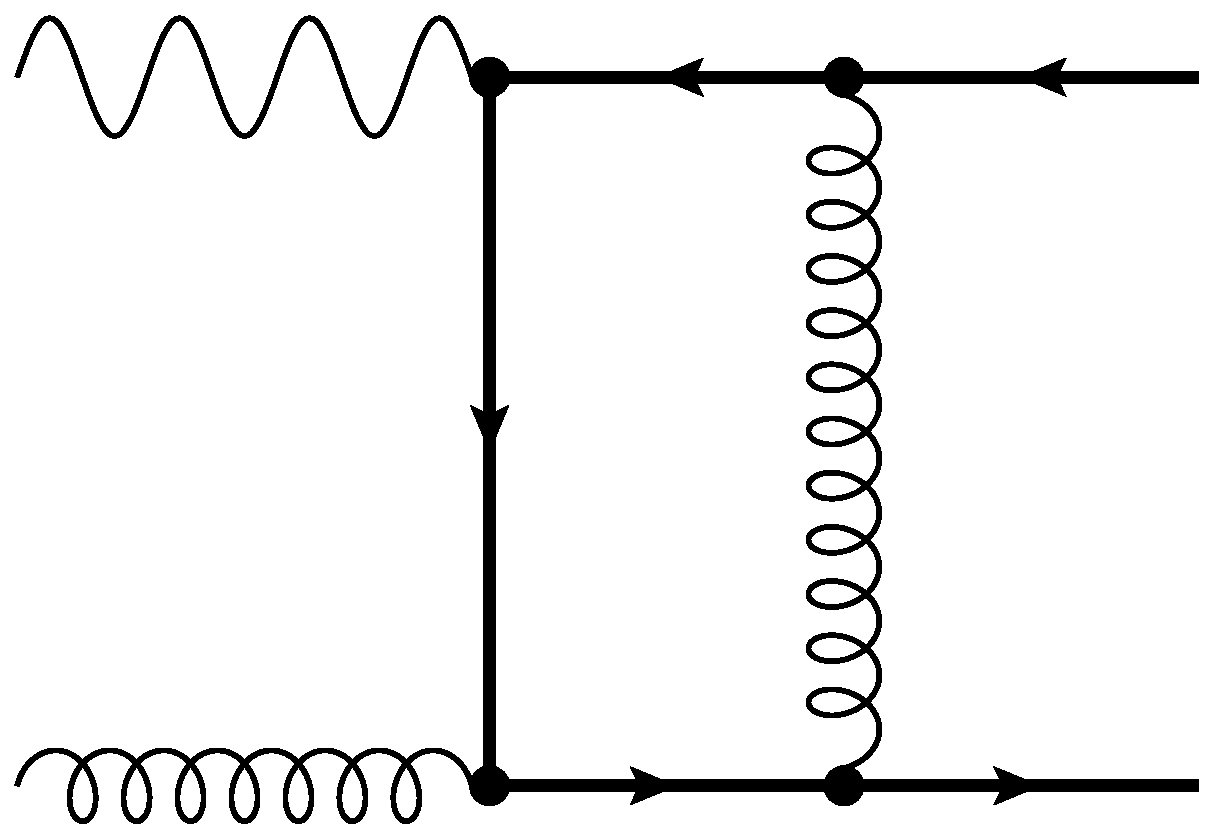
\includegraphics[width=.25\textwidth]{img/nlo-v-1}
&or
&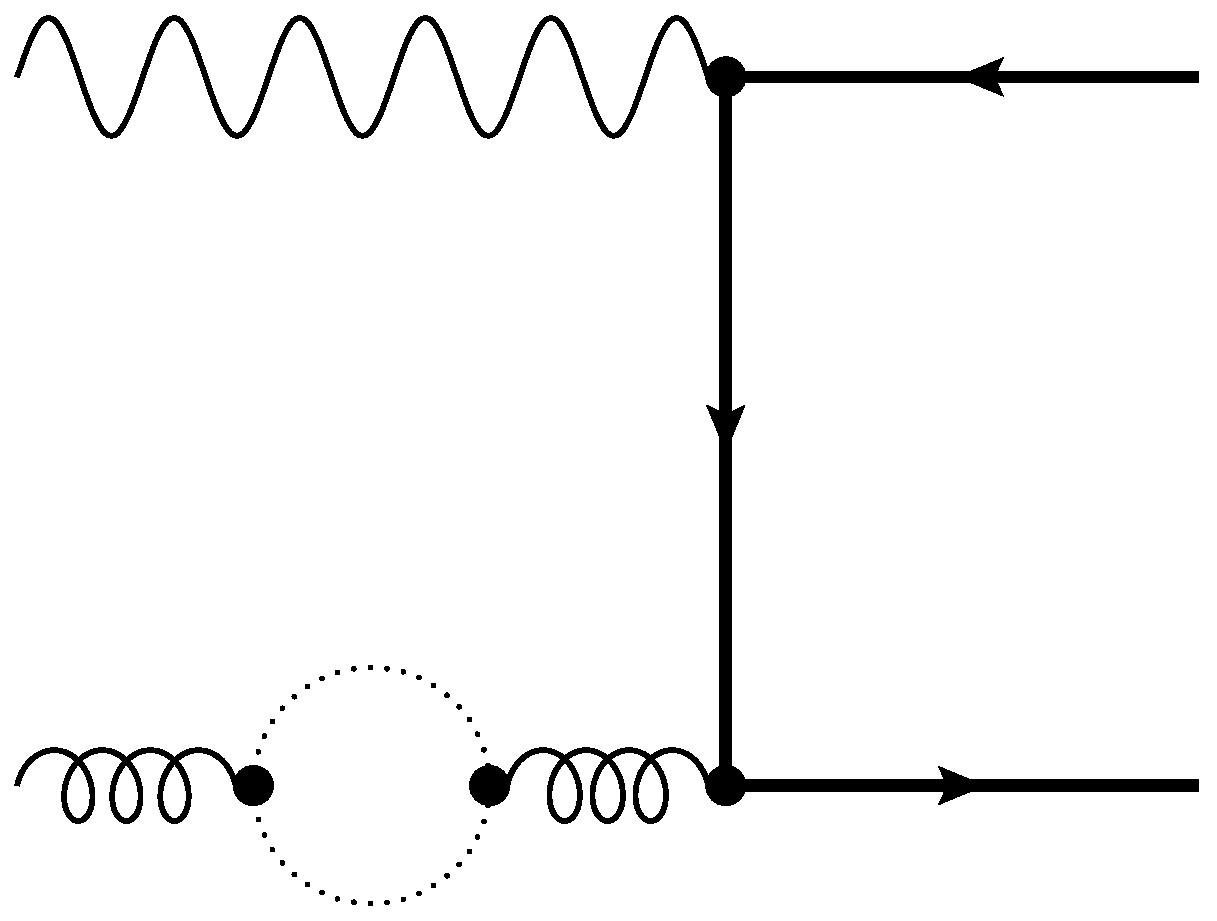
\includegraphics[width=.25\textwidth]{img/nlo-v-5}
\end{tabular}
\end{center}

soft poles appear in the limit of a soft gluon $k_2\rightarrow 0$, e.g.,
\begin{center}
\includegraphics[width=.2\textwidth]{img/nlo-g-4}
\end{center}

soft + virtual + renormalization ($\MSbar_m$) + factorization is finite!
\end{frame}

\begin{frame}[<+->]{Computation Review - Analytic Expressions}
\begin{align*}
\nonumber
&D_0(m^2,0,q^2,m^2,t,s,0,m^2,m^2,m^2) = \frac{i C_\epsilon}{\beta s t_1}\times \Bigg[ -\frac{2}{\epsilon} \ln(\chi) -2\ln(\chi)\ln\left(\frac{-t_1}{m^2}\right)\\
\nonumber
&+\DiLog(1-\chi^2)-4\zeta(2)+\ln^2(\chi_q) + 2\DiLog(-\chi\chi_q)+2\DiLog\left(\frac{-\chi}{\chi_q}\right)\\
&+2\ln(\chi\chi_q) \ln(1+\chi\chi_q)+2\ln\left(\frac{\chi}{\chi_q}\right)\ln\left(1+\frac{\chi}{\chi_q}\right) \Bigg]
\end{align*}
\begin{align*}
\nonumber
\int\!\! \frac{d\Omega_n}{t' {u_7}^2} &\sim -\frac{2 \pi  (m^2+s_4) ({s'}+{t_1}) }{s_4 {t_1}^2 {u_1}^2} \Bigg[-2+\frac{{t_1} {u_1} (-q^2 s_4+(2 m^2+s_4) ({s'}+{u_1}))}{({s'}+{t_1}) \left(q^2 s_4 {t_1}+m^2 ({s'}+{u_1})^2\right)}\nonumber\\
 & +\frac{2}{\epsilon }+\ln\left(\frac{{t_1}^2 {u_1}^2 ({m^2}+{s_4})}{({s'}+{t_1})^2 \left({m^2} ({s'}+{u_1})^2+{q^2} {t_1} {s_4}\right)}\right)\Bigg]
\end{align*}\pause
\only<beamer:2->{\begin{textblock*}{5cm}(10cm,2cm) % {block width} (coords)
\includegraphics[width=5cm]{img/c1}
\end{textblock*}}
\end{frame}
